\documentclass[letterpaper]{article}

\usepackage{gensymb}
\usepackage[vmargin=1in,hmargin=1.25in]{geometry}
\usepackage{graphicx}
\usepackage{hyperref}
\usepackage{microtype}
\usepackage{lmodern}

\author{Philip Pham}
\title{ECE/CSE 576, Spring 2019 Homework 1: Filtering, Edge finding, and Clustering}
\date{\today}

\begin{document}
\maketitle

\section*{Task 1: Convolution}

For this task, we implement a general convolution method for linear filters. My
code can be found at
\href{https://github.com/ppham27/cse576/blob/master/hw1/Code/Project1.cpp\#L216}{\texttt{Convolution}}. The
run time complexity is $O\left(HWCK_wK_h\right)$, where $H$ is the height of the
imate, $W$ is the width of the image, $C$ is the number of channels, $K_w$ is
the width of the kernel, and $K_h$ is the height of the kernel.

\section*{Task 2: Gaussian Blur}

In this task, we apply the Gaussian blur filter.

\begin{center}
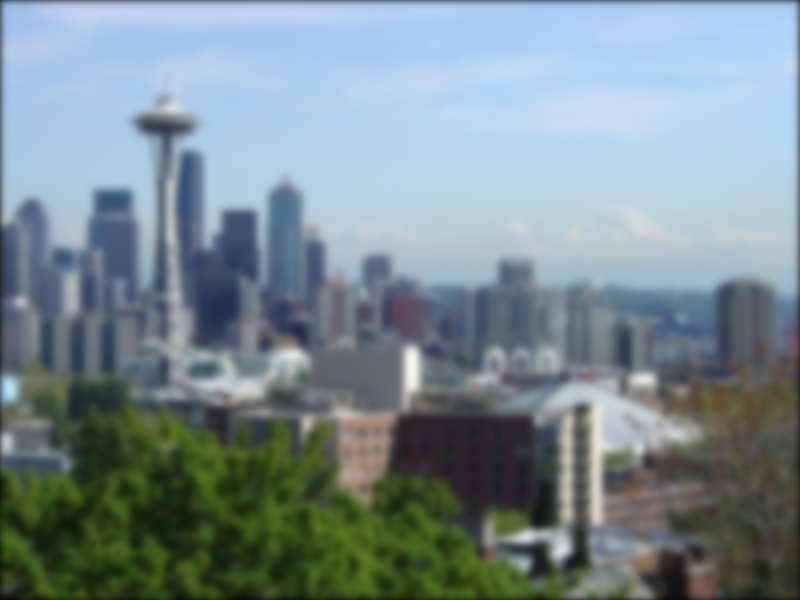
\includegraphics[width=0.85\textwidth]{task2.png}
\end{center}

$\sigma = 4.0$ was used. The darkened borders are due to zero padding.

\section*{Task 3: Separable Gaussian Blur}

The separable Gaussian blur applies a vertical and horizontal Gaussian blur
filter separately.

\begin{center}
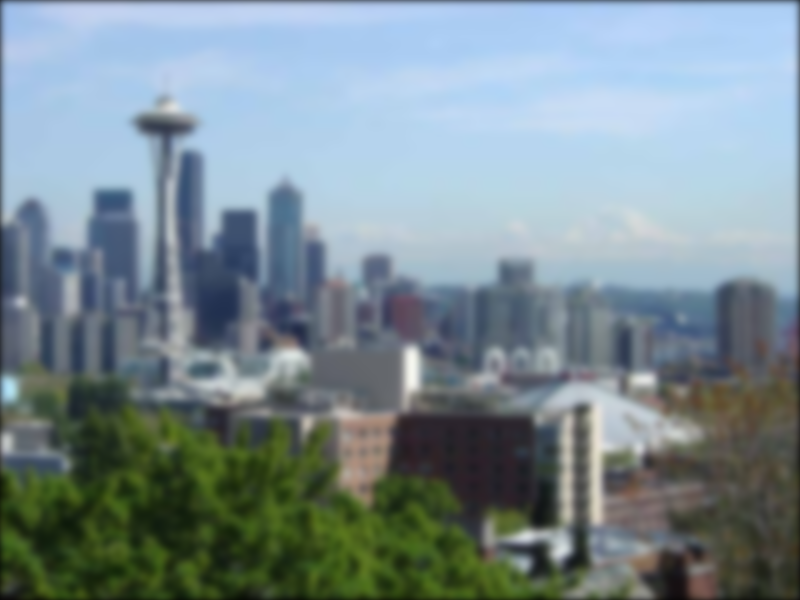
\includegraphics[width=0.85\textwidth]{task3.png}
\end{center}

The results are the same as Task 2, which demonstrates the commutativity as
associativity of convolutions.

\section*{Task 4: Image derivatives}

In this task we compute derivatives to help detect edges.

\begin{center}
  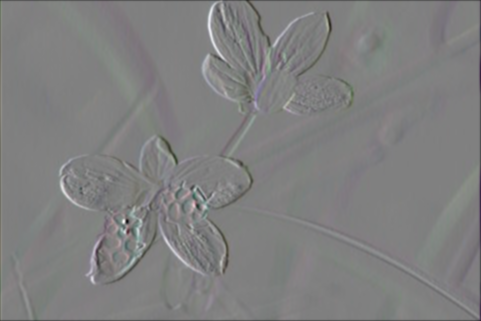
\includegraphics[width=0.85\textwidth]{task4a.png}
  
  $x$-derivative of \texttt{LadyBug.jpg} with $\sigma = 1.0$.
\end{center}

\begin{center}
  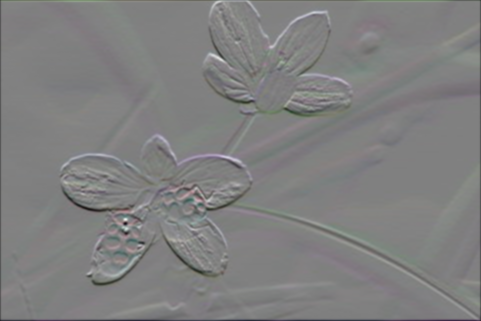
\includegraphics[width=0.85\textwidth]{task4b.png}
  
  $y$-derivative of \texttt{LadyBug.jpg} with $\sigma = 1.0$.
\end{center}

\begin{center}
  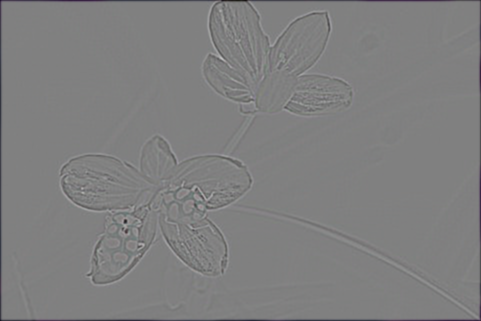
\includegraphics[width=0.85\textwidth]{task4c.png}
  
  Second derivative of \texttt{LadyBug.jpg} with $\sigma = 1.0$.
\end{center}

\section*{Task 5: Image Sharpening}

By substracting the second derivative from the original image, we can sharpen
it.

\begin{center}
  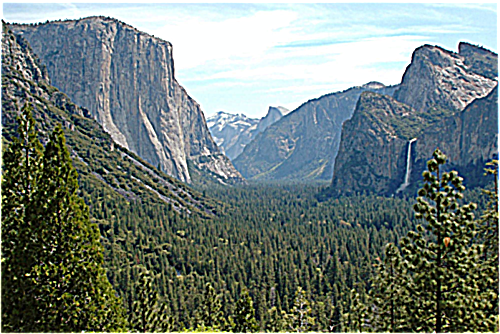
\includegraphics[width=0.85\textwidth]{task5.png}
  
  \texttt{Yosemite.png} sharpened with $\sigma = 1.0$ and $\alpha = 5.0$.
\end{center}

\section*{Task 6: Edge Detection}

The Sobel operator can be used to detect edges.

\begin{center}
  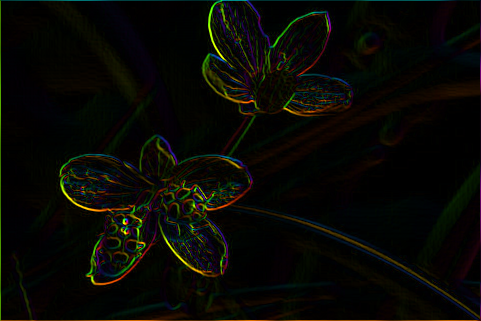
\includegraphics[width=0.85\textwidth]{task6.png}
  
  The Sobel operator is applied to \texttt{LadyBug.jpg}.
\end{center}

\section*{Task 7: Bilinear Interpolation}

Bilinear interpolation is used to rotate an image.

\begin{center}
  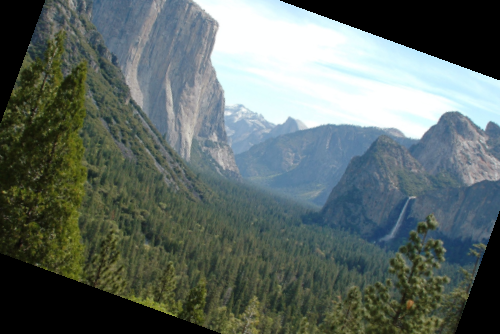
\includegraphics[width=0.9\textwidth]{task7.png}
  
  \texttt{Yosemite.png} rotated by 20\degree.
\end{center}

\section*{Task 8: Finding edge peaks}

Edge peaks are found with a combination of the Sobel operator and bilinear
interpolation. The Sobel operator gives us a pixel's magnitude and
orientation. With bilinear interpolation we can get the magnitude of the two
neighboring perpendicular pixels. If the pixel is an edge peak, it should have
the greatest magnitude.

\begin{center}
  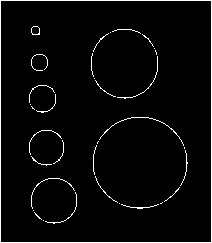
\includegraphics{task8.png}
  
  Edge peaks for \texttt{Circle.png} with a threshold of $40.0$.
\end{center}

\section*{Task 9: K-means color clustering}

Each pixel of an image can be seen as belonging to a cluster based on its
colors. Lloyd's algorithm with the $l_1$ norm is used to cluster the pixels.

\section*{Task 9a: With random seeds}

One way to initialize the clusters is randomly.

\begin{center}
  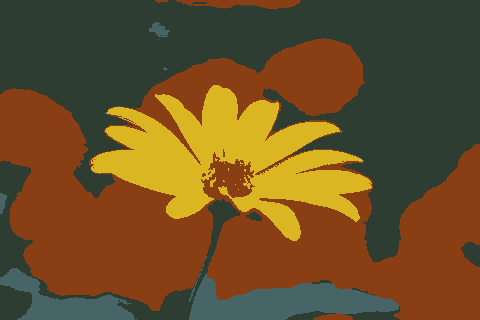
\includegraphics[width=0.85\textwidth]{task9a.png}
  
  K-means clustering applied to \texttt{Flower.png} with 4 clusters initialized
  randomly.
\end{center}

\section*{Task 9b: With pixel seeds}

Another way to initialize the clusters is by selecting a subset of pixels to be
initial seeds.

\begin{center}
  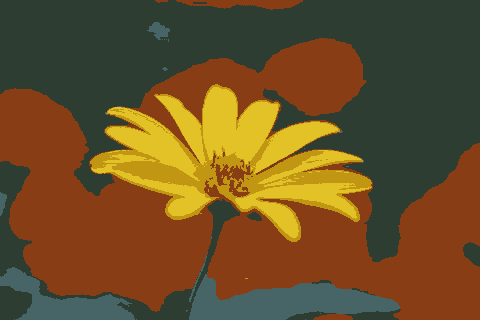
\includegraphics[width=0.85\textwidth]{task9b.png}
  
  K-means clustering applied to \texttt{Flower.png} with 5 clusters initialized
  from pixel seeds.
\end{center}

\section*{Bells: Reflected padding}

As seen in Tasks 2 and 3, one downside of zero padding is that the intensity of
the border points change. Padding by reflecting along the image borders can fix
this.

\begin{center}
  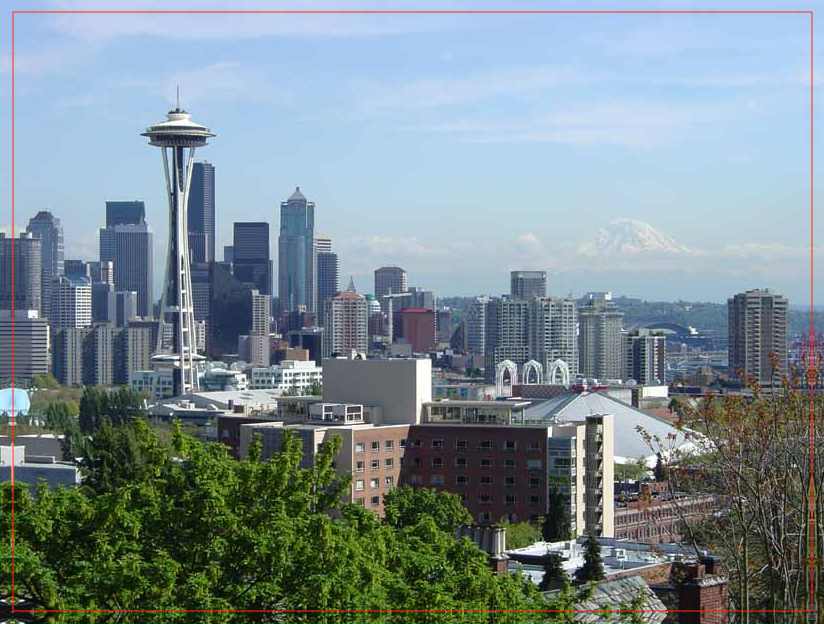
\includegraphics[width=0.824\textwidth]{reflectedpaddingtaskborder.png}
  
  \texttt{Seattle.jpg} padded out. The original border is shown in red.
\end{center}

\begin{center}
  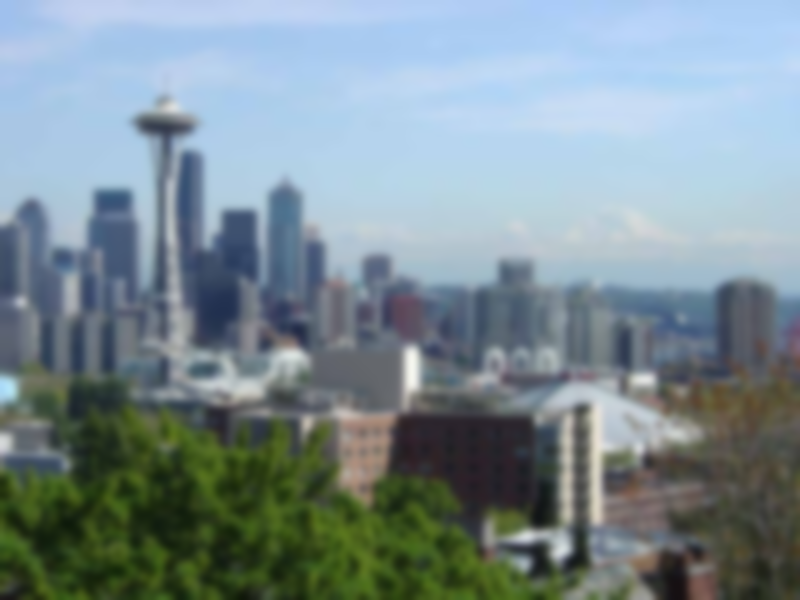
\includegraphics[width=0.8\textwidth]{reflectedgaussianblur.png}
  
  Gaussian blur with $\sigma = 4.0$ applied to a padded with reflection \texttt{Seattle.jpg}.
\end{center}

The pixel intensity along the border is now maintained in constrast to Tasks 2 and 3.

\section*{Bells: Histogram K-means}

In Task 9b, selecting clusters from the empirical distribution of pixels can be
noisy. One way to smooth out the distribution is to bucket them into a histogram
and initialize clusters that way. If each color is divided into $8$ buckets,
there will be $8 \times 8 \times 8 = 512$ total buckets.

\begin{center}
  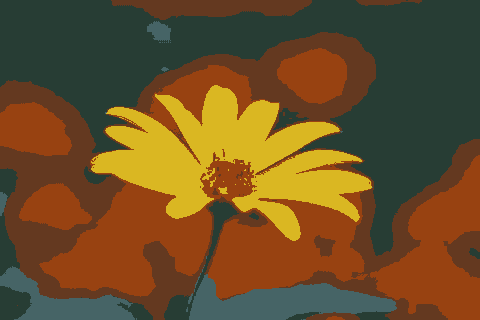
\includegraphics[width=0.85\textwidth]{histogramtask.png}
  
  K-means clustering of \texttt{Flower.png} into 5 clusters initialized from a
  histogram.
\end{center}

\section*{Bells: Median Filter}

Taking the median intensity of of a neighborhood can smooth and reduce noise.

\begin{center}
  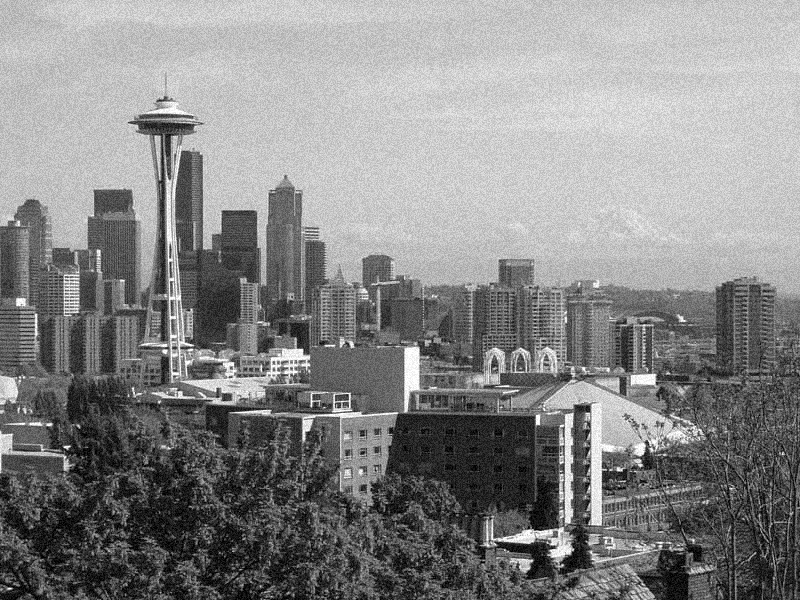
\includegraphics[width=0.7\textwidth]{mediantasknoise.png}

  Noisy black and white version of \texttt{Seattle.jpg}.
  
  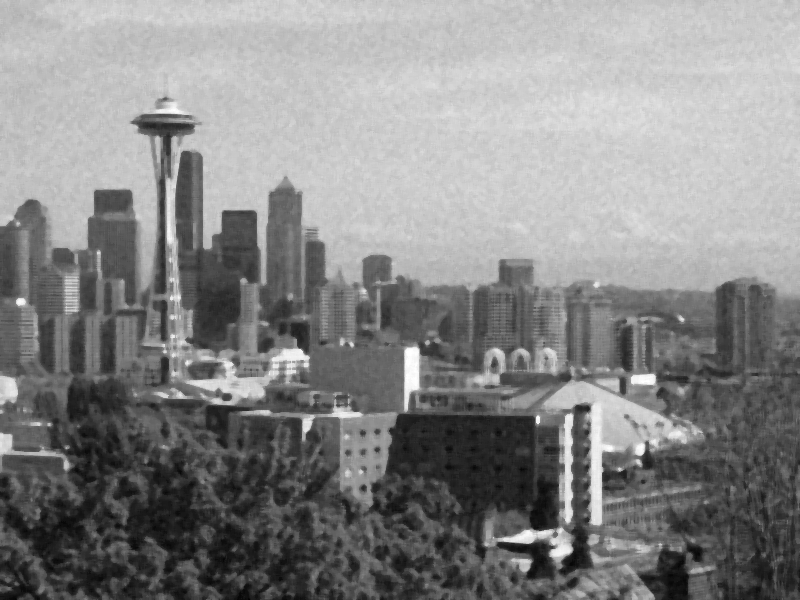
\includegraphics[width=0.7\textwidth]{mediantask.png}
  
  Noise reduction on greyscale version of \texttt{Seattle.jpg} with a median
  filter of radius 2.
\end{center}

\section*{Whistles: Bilateral Filter}

The bilateral filter is similar to the Gaussian filter in that it smooths and
reduces noise. By using a weighted average of pixel intensity, it preserves
sharp edges.

\begin{center}
  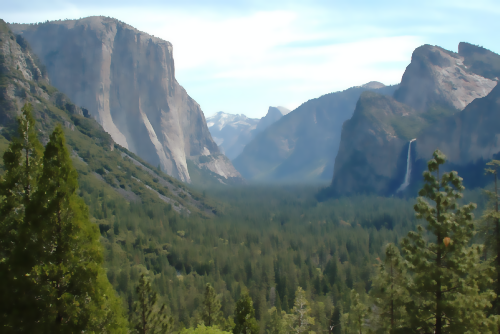
\includegraphics[width=0.85\textwidth]{bilateraltask.png}

  Bilateral filter applied to \texttt{Yosemite.png} with $\sigma_S = 2.0$ and
  $\sigma_I = 20.0$.
\end{center}

\section*{Whistles: Hough Transform}

The Hough transform takesas input edge peaks. For each edge peak pixel, the
Hough transform considers all the lines that the pixel could possibly be part of
by considering all $\theta$ in polar $\left(r, \theta\right)$ space. The most
likely lines are returned and merged with the edge peaks are filtered based on
these lines to get line segments.

\begin{center}
  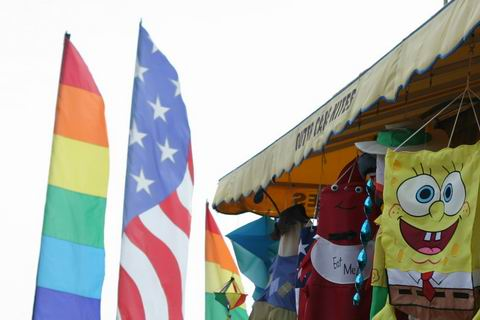
\includegraphics[width=0.6\textwidth]{houghtask1.png}
  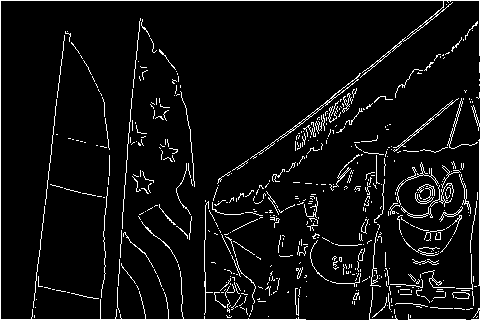
\includegraphics[width=0.6\textwidth]{houghtask2.png}
  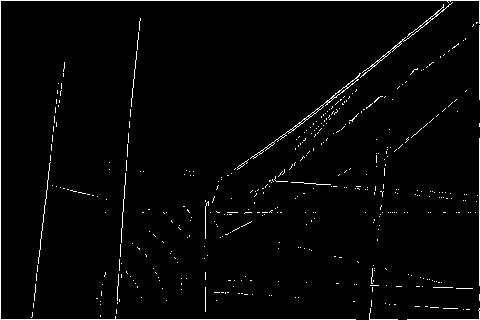
\includegraphics[width=0.6\textwidth]{houghtask3.png}

  Identifying line segments with the Hough transform in \texttt{Flags.png}. The
  original image, edge peaks, and the result of the Hough transform are shown.
\end{center}

\section*{Appendix}

All code used to generate these images can be found at
\href{https://github.com/ppham27/cse576/blob/master/hw1}{\texttt{ppham27/cse576/hw1}}. The
embedded PNG files and the \LaTeX can be found in
\href{https://github.com/ppham27/cse576/blob/master/hw1/report}{\texttt{ppham27/cse576/hw1/report}}.

\end{document}
